\subsubsection{Licence}
GNU GPLv2.\\

Notice de copyright dans le code source :
{\small
\begin{verbatim}
 * Trampoline RTOS
 *
 * Trampoline is copyright (c) CNRS, University of Nantes, Ecole Centrale de Nantes
 * Trampoline is protected by the French intellectual property law.
 *
 * This software is distributed under the GNU Public Licence V2.
 * Check the LICENSE file in the root directory of Trampoline
 *
\end{verbatim}
}

\subsubsection{Code source}
Dépôt github.com : \url{https://github.com/TrampolineRTOS/trampoline}.\\

Tags Doxygen présents dans les commentaires.\\

Le code est un peu bizarre :
\begin{verbatim}
/*
 * MISRA RULE 13 VIOLATION: this function is only used for debug purpose,
 * so production release is not impacted by MISRA rules violated
 * in this function
 */
FUNC(void, OS_CODE) printrl(P2VAR(char, AUTOMATIC, OS_APPL_DATA) msg)
{
\end{verbatim}

Il semble qu'il respecte la norme de programmation MISRA C de la \emph{Motor Industry 
Software Reliability Association} que l'on peu ce procurer pour 45£.\\

Il utilise également le langage de description d'application OIL (Figure 
\ref{fig:oil}).

\begin{figure}[!h]
	\begin{center}
		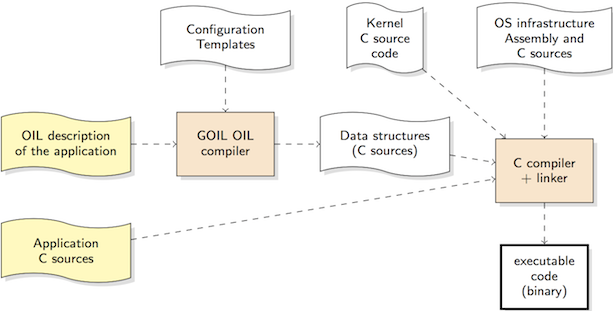
\includegraphics[scale=2.5]{images/trampoline_building.png}
	\end{center}
	\caption[]{\label{fig:oil} The building process of the executable of an
				application using Trampoline \cite{ref7}.}
\end{figure}

\subsubsection{Plateformes cible}
Il a été porté sur STM32F4 Discovery :
\url{https://github.com/TrampolineRTOS/trampoline/wiki/The-STM32F4-Discovery-port}

\subsubsection{Communauté}
Le projet semble entièrement hébergé sur github.com avec actuellement 13
contributeurs. Il y a eu 2682 commits depuis 2006, le dernier date d'il y a 10 jours.
\\

Le wiki contient 16 pages. La page d'accueil donne une description succincte du
projet :
{\small
\begin{verbatim}
Trampoline is a Real Time Operating System (RTOS) which is developed by the Real Time
System Group at LS2N (ex-IRCCyN) Laboratory (France). Trampoline implements the OSEK
and AUTOSAR standards.
\end{verbatim}
}
\subsubsection{Acceptabilité}
\begin{tabular}{lll}
\toprule
	Critère				&	Validé		&	Commentaire	\\
\midrule
	Licence				&	oui			&	+ copyright CNRS	\\
	Code source			&	non			&	MISRA C non libre	\\
	Plateformes cible	&	oui			&	STM32F4	\\
	Communauté			&	non			&	insuffisante	\\
\bottomrule
\end{tabular}

